
\chapter{Przegląd zagadnień teoretycznych}

\section{Zarys działania Microsoft DirectX API}

\subsection{Struktura i podstawowe pojęcia}

Microsoft DirectX to interfejs programistyczny (API, ang. \emph{application programming interface}) do tworzenia aplikacji multimedialnych. Składają się na nie przede wszystkim:

\begin{itemize}
\item DirectDraw, Direct2D/Direct3D (komponenty odpowiedzialne za rysowanie grafiki),
\item DirectSound, DirectMusic (obsługa dźwięków),
\item DirectInput (obsługa wejścia - myszy, klawiatury, kontrolerów itp.).
\end{itemize}

DirectX pozwala na tworzenie aplikacji w trzech językach - C\#, Visual Basic oraz C++, przy czym w praktyce spotyka się głównie aplikacje stworzone w C\# oraz C++.
Jak widać na rysunku \ref{directx_infrastructure}, struktura DirectX jest wielopoziomowa i, poza odwołaniami do API oraz komponentami jak na przykład Direct3D 11 (D3D11), obejmuje także DXGI (Infrastruktura Graficzna DirectX, ang. \emph{Microsoft DirectX Graphics Infrastructure}), które -- jako najniższa warstwa -- komunikuje się bezpośrednio ze sterownikiem znajdującym się w przestrzeni jądra systemu operacyjnego. Wykorzystanie komponentów COM (ang. \emph{Component Object Model}) pozwala na łatwą rozbudowę oraz jasny podział funkcjonalności.\\
\begin{figure}
\begin{center}
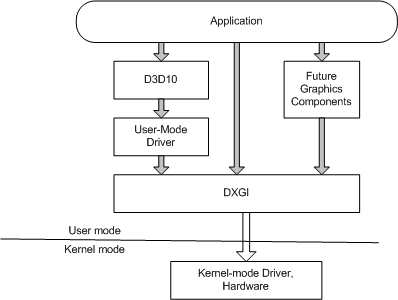
\includegraphics[scale=0.4]{figures/directx_infrastructure.png}
\caption{Architektura DirectX}
\label{directx_infrastructure}
\end{center}
\end{figure}
Podstawowymi i koniecznymi do zrozumienia działania DirectX są koncepcje urządzenia (ang. \emph{device}) oraz jego kontekstu (ang. \emph{device context}).\\
Urządzenie, reprezentowane w~wersji 11. przez interfejs ID3D11Device, reprezentuje kartę graficzną i może służyć do tworzenia zasobów oraz pobierania informacji o~jej możliwościach (ang. \emph{capabilities}), tj. oferowanych przez nią funkcjonalnościach takich jak np. obsługa podwójnej precyzji w~programach cieniujących.\\
Kontekst urządzenia z kolei, jak wskazuje nazwa, określa kontekst użycia urządzenia, co jednoznacznie pokazuje, iż do prawidłowej pracy z~urządzeniem powiązany powinien być co najmniej jeden kontekst. Pozwala on głównie na ustawienie stanu w~procesie renderingu oraz prawidłowych komend wykorzystujących zasoby karty graficznej do wygenerowania obrazu (bezpośrednio na ekran lub do pośredniczącej tekstury, która może zostać wykorzystana później). Wyróżniamy dwa rodzaje kontekstów: bezpośredni/zwykły (\emph{forward}) oraz opóźniony (\emph{deferred}). Bezpośredni wykonuje komendy od razu gdy zostają wywołane, podczas gdy opóźniony pozwala na zapisanie ich na odpowiedniej liście, dzięki czemu mogą zostać wykonane później (jest to przydatne zwłaszcza w przypadku aplikacji wielowątkowych).\\

\subsection{Proces renderingu}

Przebieg wygenerowania grafiki (renderingu) opisywany przez tzw. \emph{pipeline} jest złożony z~wielu etapów (ang. \emph{stage}), z~których część może być konfigurowana jedynie przez wywołanie odpowiednich komend API poprzedzonych prefiksem będącym skrótem nazwy danego etapu (np. \emph{IA} dla etapu \emph{Input-Assembler}), a część opisywana jest przez programy cieniujące (ang. \emph{shader}).\\
W pipeline DirectX 11 wyróżnia się następujące etapy:
\begin{itemize}
\item Input-Assembler - odpowiada za wczytanie wierzchołków w~sposób opisany przez prymityw (trójkąt, czworokąt itp.),
\item Vertex Shader - cieniowanie wierzchołków, ustalanie dla nich wartości początkowych zmiennych jak np. kolor, wektor normalny itp. ,
\item Hull Shader - pierwszy etap teselacji (zagęszczania siatki), przygotowuje siatkę do zagęszczenia przez ustalenie punktów kontrolnych,
\item Tessellator - zagęszcza siatkę wprowadzając dodatkowe prymitywy zastępujące podstawowy i zwraca nowe współrzędne teksturowania,
\item Domain Shader - generuje nowe pozycje wierzchołków na podstawie dwóch poprzednich etapów,
\item Geometry Shader - pozwala zastąpić prymityw wejściowy innym prymitywem,
\item Rasterizer - odpowiada za "spłaszczenie" obrazu tak, aby mógł zostać wyświetlony na ekranie,
\item Pixel Shader - pozwala zmieniać kolor piksela w~wynikowym obrazie,
\item Output Merger - generuje końcowy obraz łącząc w~odpowiedni sposób (opisany przez komendy takie jak np. OMSetRenderTargets) informacje z~poprzedniego etapu.
\end{itemize}

Wszystkie te etapy przedstawione zostały na Rys. \ref{directx_pipeline}. Strzałki określają czy dany etap korzysta jedynie z odczytu danych z karty, czy też pozwala na ich zapis (lub oba równocześnie).

\begin{figure}
\begin{center}
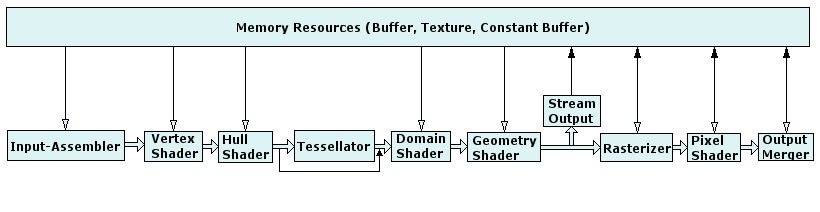
\includegraphics[scale=0.5]{figures/directx_pipeline.png}
\caption{Proces generowania obrazu w DirectX}
\label{directx_pipeline}
\end{center}
\end{figure}

Ostatnim zasługującym na uwagę jest fakt, iż w~większości aplikacji wraz z DirectX wykorzystywana jest technologia WinAPI pozwalająca na tworzenie aplikacji graficznych pod platformę Windows. Głównym jej mechanizmem jest pętla komunikatów, których odebranie warunkuje sposób przetwarzania informacji w aplikacji (np. wciśnięcie klawisza powoduje przesunięcie modelu). Komunikaty mogą zostać odczytane w sposób blokujący (przez funkcję \emph{GetMessage}) lub nieblokujący (\emph{PeekMessage}). Z~oczywistych względów (tj. narzutu czasowego), w~aplikacjach generujących obraz w~czasie rzeczywistym wykorzystywana jest wyłącznie funkcja nieblokująca.

\section{Deferred Shading}

Podstawowym sposobem obliczania oświetlenia, uwzględniając opisany wcześniej proces generacji obrazu, jest wyliczenie oświetlenia bezpośrednio dla każdego obiektu. Wartości takie jak wektory normalne, współrzędne teksturowania i inne używane we~wspomnianym procesie są wczytywane w shaderze wierzchołków, a następnie interpolowane we~fragment/pixel shaderze. W~przypadku wielu źródeł oświetlenia (na przykład 2000 lub więcej), dla każdego obiektu (niezależnie od tego, czy jest widoczny) należy sprawdzić wszystkie źródła światła, co oznacza złożoność
\begin{equation}
\label{forward_shading_complexity}
O(~liczba\_pikseli\_per\_obiekt~*~liczba\_zrodel\_swiatla~)
\end{equation}
co z~kolei w wielu przypadkach jest nie do zaakceptowania (z~\ref{forward_shading_complexity} wynika, iż zwiększanie liczby obiektów zmniejsza liczbę źródeł światła, których można użyć na scenie).\\
Jeśli jednak proces obliczania oświetlania przesuniemy do oddzielnego etapu następującego po wyliczeniu tego, które obiekty są aktualnie widoczne, otrzymamy złożoność
\begin{equation}
\label{deferred_shading_complexity}
O(~liczba\_pikseli~*~liczba\_zrodel\_swiatla~)
\end{equation}
Jak z kolei widać z~\ref{deferred_shading_complexity}, podejście to nie wprowadza już zależności między liczbą obiektów a liczbą źródeł światła. Pozwala to uzyskać o wiele lepszą wydajność w przypadku scen z wieloma złożonymi obiektami oraz złożonym oświetleniem. Możliwe jest również wprowadzenie wielu uprawnień, jak na przykład podział obrazu na wiele "kafelków" (ang. \emph{tile}), z których każda może zostać obliczona przez wątki na karcie graficznej - technika ta nosi nazwę \emph{tiled deferred rendering} i jest powszechnie stosowana w~popularnych silnikach graficznych.\\
Uzyskanie tego efektu wymaga utworzenia kilku tekstur pośredniczących, które łącznie noszą nazwę \emph{G-Buffera}. Jest on wykorzystywany do przetrzymywania efektów pośrednich procesu renderingu oraz wyliczenia obrazu końcowego. Format G-Buffera zmienia się w~zależności od zastosowania oraz algorytmu obliczania oświetlenia i osoby odpowiadającej za jego implementację, jednak najczęściej wykorzystywane są tekstury:
\begin{itemize}
\item wektorów normalnych,
\item koloru/albedo,
\item głębokości.
\end{itemize}
Pomimo wielu zalet, deferred shading ma jednak swoje wady. Obliczanie oświetlenia z gotowego obrazu uniemożliwia łatwe obliczenie kolorów w przypadku przezroczystych obiektów, zaś wyświetlanie obrazu końcowego w postaci tekstury wymaga wykorzystania bardziej skomplikowanych algorytmów obliczania antyaliasingu, co z~kolei obciąża kartę graficzną. Mimo to deferred shading, w zmodyfikowanych odmianach, jest powszechnie wykorzystywany w~wielu popularnych grach komputerowych oraz innych aplikacjach renderujących obraz w~czasie rzeczywistym.

\section{Podpowierzchniowe Rozproszenie Światła/Rozpraszanie Podpowierzchniowe (SubSurface Scattering)}

Kolory obserwowane na co dzień są efektem odbicia fotonów od powierzchni obserwowanego obiektu (oraz innych obiektów, co skutkuje efektem tak zwanego "krwawienia kolorów" (ang. \emph{color bleeding}, czyli zabarwienia obiektu kolorem światła odbitego). Jeśli jednak światło zamiast odbić się bezpośrednio dostanie się pod powierzchnię obiektu, odbije kilka razy wewnątrz i wyjdzie w innym punkcie, to zobaczymy, iż obiekt ten jest półprzezroczysty - światło dociera jedynie na pewną głębokość określaną mianem promienia rozproszenia światła (ang. \emph{scattering radius}), gdzie zostaje zabarwione na nowy kolor. Przykładem materiałów zachowujących się w ten sposób mogą być wosk, mleko, marmur czy skóra.\\
Efekt ten jest trudny do obliczenia w czasie rzeczywistym, w związku z czym w większości przypadków stosuje się jedynie pewne przybliżenia. Przykładem algorytmu dającego przybliżone lecz skuteczne rozwiązanie jest wykorzystanie map głębokości. Opiera się on na zasadzie podobnej do obliczania map cieni (ang. \emph{shadow maps}), jednak w tym wypadku z punktu widzenia źródła światła zapisuje się bardziej skomplikowaną informację - drogę, jaką musi pokonać światło przechodząc przez obiekt, a więc odległość pomiędzy dwoma punktami leżącymi na jego powierzchni z obu stron obiektu. Podczas kolejnego przejścia procesu renderingu można wykorzystać tę informację do oszacowania koloru wynikowego.

\section{Głębia Ostrości (Depth of Field)}

Ostatnim teoretycznym zagadnieniem objaśnianym w tym rozdziale jest zjawisko głębi ostrości, znane powszechnie między innymi z fotografii. Jak opisano w \cite{gpugems_23}, polega ono na skupieniu ostrości na pewnym obiekcie lub grupie obiektów w zależności od ogniskowej soczewki, przesłony oraz tak zwanego "krążka rozmycia" (ang. \emph{circle of confusion}; jest to parametr wpływający na ogólną ostrość/rozmycie obrazu).\\
Ponieważ istnieje wiele algorytmów obliczania głębi ostrości, a sam proces wyznaczania potrzebnych wartości jest skomplikowany, nie będzie on opisywany w niniejszej pracy.
